% IMMI-formatted version of the projection-law paper.
% Format-free initial submission per Springer practice; structured abstract,
% numbered citations, single column, declarations block per IMMI conventions.
% The PRX-formatted master is ../projection-law.tex --- kept in sync with
% the June 14, 2026 revision.
\documentclass[11pt]{article}
\usepackage[utf8]{inputenc}
\usepackage[T1]{fontenc}
\usepackage{amsmath,amssymb,amsthm}
\usepackage{booktabs}
\usepackage{tabularx}
\usepackage{graphicx}
\usepackage[margin=2.5cm]{geometry}
\usepackage[numbers,sort&compress]{natbib}
\usepackage[hyphens]{url}
\usepackage{hyperref}
\hypersetup{colorlinks=true, linkcolor=blue, citecolor=blue, urlcolor=cyan}
\graphicspath{{../figures/}}

\newtheorem{theorem}{Theorem}
\newtheorem{corollary}{Corollary}
\theoremstyle{remark}
\newtheorem{remark}{Remark}
\newcommand{\inn}[2]{\langle #1, #2 \rangle}

\title{\bfseries The Projection Law: Model-Ensemble Errors Point at Their Binding Constraint}
\author{Alex Welcing\\ \small Lupine Science, Union City, NJ\\ \small \texttt{alexwelcing@gmail.com}\\ \small ORCID: \href{https://orcid.org/0009-0002-1602-8545}{0009-0002-1602-8545}}
\date{June 29, 2026}

\begin{document}
\maketitle

\begin{abstract}
\noindent\textbf{Purpose:} Multi-model agreement is routinely used as
confidence in materials simulation and beyond, yet models in a family share
construction and training lineage. This work formalizes and tests the
projection law: a model family acts as a projection operator, every
well-fitted member shares one residual --- a single direction in observable
space --- and that direction fingerprints whatever constraint binds the
family.
\textbf{Methods:} The theoretical core --- normal-cone consensus on convex
families, a closed-form participation-ratio gauge, and a pointwise local
normal-cone theorem for smooth non-convex families --- is machine-checked in
Lean~4 with zero unproven obligations. The
\emph{formal} theorems cover convex (and locally smooth) reachable sets; their
application to non-convex neural-network families is an empirical regularity
tested below, not a mathematical consequence of the theorems. Two factorial
experiments were pre-registered with refutation conditions committed before
execution: a $4{\times}2$ architecture-by-functional crossing of MatPES-trained
foundation interatomic potentials evaluated on elastic constants of 15 cubic
metals, and an analysis of 12 DFT implementations on 384 equation-of-state
benchmarks from the ACWF verification effort. A two-tier replication kit
verifies every statistic from committed raw data (NumPy only, seconds) and
re-derives the raw data from public checkpoints (deterministic within 1~GPa;
the Gate-0 harness regression is bit-exact).
\textbf{Results:} In the foundation-model layer the \emph{direction} of the
prediction is confirmed but its \emph{magnitude} is weak: errors cluster by
training functional rather than architecture ($S_{\mathrm{func}}{=}{+}0.317$
vs.\ $S_{\mathrm{arch}}{=}{-}0.093$), yet the exact permutation test sits at the
lattice's resolution floor ($p{=}0.029$, 2 of 70 labelings) and the registered
effect-size component \emph{failed} ($0.085$ vs.\ the registered $0.30$); the
rotation prediction was confirmed on Au and Pt under r$^2$SCAN but not Ag. We
report this conjunctive test as a failure, not a partial success. These Layer~2
errors are measured against mixed references (experimental for FCC metals,
DFT-PBE for others), so the residual convolves fitting error with
exchange--correlation bias and thermal/zero-point offsets; a registered 0~K
DFT-PBE elastic anchor (round~2) is the decisive test that separates them. DFT
implementation errors, by contrast, cluster by pseudopotential table, not
simulation code ($S_{\mathrm{table}}{=}{+}0.526$ vs.\
$S_{\mathrm{code}}{=}{+}0.265$, $p{=}0.017$); four independent plane-wave codes
sharing one table align at $0.70$--$0.87$. Neither registered refutation
condition was triggered, but four of seven registered predictions failed and are
reported as failures.
Combined with the 559-potential classical baseline (within-family
reference--prediction correlation $0.95$; error dimensionality invariant over
forty years), error anisotropy is conserved across paradigm replacements while
its direction rotates to the next constraint upstream. A correction direction
fitted with the corrected model held out removes a median $69\%$ of
foundation-model squared elastic error out-of-sample (IQR $35$--$92\%$;
per-element medians up to $97\%$).
A new Round-2 $3{\times}3{\times}3$ benchmark of $16$ cubic metals with four
MatPES foundation MLIPs validates a one-vector-per-functional
leave-one-out correction operator that reduces mean absolute elastic error
from $17.84$~GPa to $10.36$~GPa with zero no-harm violations, improving
every architecture on both PBE and approximate r$^2$SCAN targets.
Pre-registered functional-clustering hypotheses H1 and H2a fail on the
$3d$/$4d$ subset, while the operator-vs-ensemble head-to-head passes on
MAE but not on conformal coverage; these mixed results point to a
bonding-class-aware operator and a direct A6 bridge test as the next step.
The corrected C$_{ij}$ MAE is an empirical oracle aggregate and is
\textbf{uncertified} as a correction license unless $C_{11}$, $C_{12}$, and
$C_{44}$ each satisfy a valid held-out-target license. Derived moduli and
composites are likewise uncertified because componentwise licenses do not
compose through differences, mixed directions, or general products.
\textbf{Conclusion:} Agreement among models sharing a constraint measures the
constraint, not the truth. Error-vector geometry converts benchmarking from
scoring into diagnosis, supplies a zero-cost trust rule for ensemble
uncertainty, and enables family-level calibration without retraining.
\end{abstract}

\noindent\textbf{Keywords:} model ensembles; error geometry; uncertainty
quantification; interatomic potentials; foundation models; density functional
theory; verification and validation; benchmarking; formal methods

\section{Introduction}

Every field that builds models in families uses inter-model agreement as
evidence. The practice has long been questioned qualitatively: climate
ensembles share construction and history, so their consensus may reflect
common structure rather than truth \citep{pirtle2010,parker2011}, and error
correlations between members quantify that dependence
\citep{bishop2013,annan2011,knutti2013}. In machine learning, independently
trained networks agree far beyond what their accuracy predicts
\citep{mania2019,geirhos2020}, ensemble members cluster in prediction space
\citep{fort2019}, and disagreement tracks the shared bias of the training
procedure rather than correctness \citep{jiang2021}. What these literatures
establish qualitatively, this paper makes geometric, formal, and---in the
specific sense of identifying \emph{which} constraint binds---operational.

The central object is the \emph{error vector}: for model $i$ in family $F$
evaluated on observables with reference values, $e_i \in \mathbb{R}^d$ is the
vector of (relative) errors. The law has three parts:

\textbf{(i) Projection.} A model family is a projection operator. Fitting,
however performed and by whomever, drives predictions toward the point of the
family's reachable set nearest the truth; the residual is a property of the
\emph{(family, target)} pair, not of any individual model or modeler. All
well-fitted members therefore share one residual direction
(Theorems~\ref{thm:cone}--\ref{thm:consensus}).

\textbf{(ii) Gauge.} The ensemble's error second moment is a shared bias plus
fitting noise; its participation ratio is a closed-form gauge of the
systematic fraction (Theorem~\ref{thm:gauge}), so low error dimensionality is
not a curiosity but a necessity for any converged family, at an explicit rate.

\textbf{(iii) Conservation and rotation.} When a modeling paradigm is
replaced --- when the binding constraint is removed --- the error anisotropy
does not dissolve into isotropic scatter. It is conserved, and its direction
rotates to the next constraint upstream in the epistemic stack
(Fig.~\ref{fig:law}a). This is the part of the law for which we find no
antecedent in the climate, forecasting, machine learning, or materials
literatures, and it is the part we test hardest (Fig.~\ref{fig:law}b).

\begin{figure}[t]
\centering
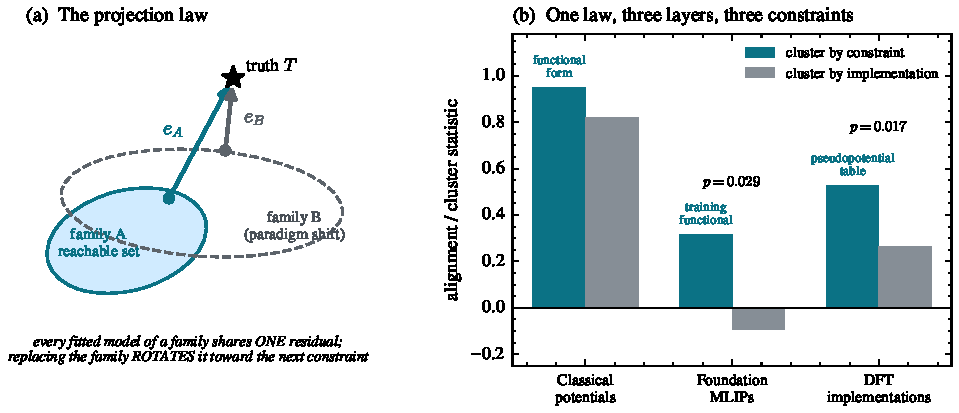
\includegraphics[width=\textwidth]{fig1_law_and_stack.pdf}
\caption{\textbf{The projection law and its three-layer test.}
(a)~A model family's reachable set fixes the residual of every well-fitted
member (Theorems~\ref{thm:cone}--\ref{thm:consensus}); replacing the family
(paradigm shift) rotates the shared residual rather than removing it.
(b)~Cluster-by-constraint versus cluster-by-implementation statistics at
three layers of one epistemic stack, plotted on a common ``alignment'' axis
whose definition differs by layer and is stated in each panel: Layer~1 uses the
Pearson correlation of scalar error \emph{norms} (reference--prediction, an
observational magnitude statistic, $r{=}0.95$); Layers~2--3 use the mean
error-\emph{vector} cosine, a directional statistic ($S_{\mathrm{func}}$,
$S_{\mathrm{arch}}$, $S_{\mathrm{table}}$, $S_{\mathrm{code}}$). The two are not
numerically commensurate and are not pooled: the gauge
$\mathrm{PR}(d,\rho)$ of Theorem~\ref{thm:gauge} is what relates magnitude order
(Layer~1) to directional collapse (Layers~2--3). Layers~2--3 show the
pre-registered cluster statistics with exact permutation $p$-values; the
registered refutation condition (implementation $>$ constraint) was not
triggered in either experiment.}
\label{fig:law}
\end{figure}

We instantiate the law at three layers of a single epistemic stack ---
classical interatomic potentials, foundation machine-learned interatomic
potentials (MLIPs), and the density-functional-theory (DFT) implementations
that generate their training data --- because this stack offers what few
domains can: large open model ensembles, factorial structure (the same
architecture trained on two functionals; the same simulation code run with two
pseudopotential families), and references at every layer. The empirical
discovery paper for the first layer is reported separately
\citep{welcing2026instance}; here that layer serves as the observational base
of a cross-layer test.

Three methodological commitments distinguish this work. The theory core is
\emph{machine-checked}: every theorem below is verified in Lean~4 with zero
unproven obligations, and a written contract maps each theorem to the
statistic that instantiates it. The two new experiments are
\emph{pre-registered}, with thresholds and explicit refutation conditions
committed to version control before any model was executed; we report all
threshold misses as failures. And the entire evidence chain is packaged for
\emph{tiered replication}: the analysis layer verifies from committed raw data
with no machine-learning dependencies in seconds, and the physics layer
re-derives the raw data from public checkpoints deterministically (within
1~GPa tolerance; the harness regression itself is bit-exact).

\section{Theoretical framework}
\label{sec:theory}

The mathematics of best approximation is classical
\citep{deutsch2001,kinderlehrer1980}; we claim only its epistemic application
to model ensembles and the machine-checked instantiation chain. Throughout,
$E$ is a real inner-product space (observable space), $s \subseteq E$ a model
family's reachable set, $T \in E$ the truth.

\begin{theorem}[Normal-cone criterion]\label{thm:cone}
Let $s$ be convex and $p$ a best approximation of $T$ in $s$
(i.e.\ $p \in s$ and $\|T-p\| \le \|T-q\|$ for all $q \in s$). Then the
residual $T - p$ lies in the normal cone of $s$ at $p$:
$\inn{T-p}{q-p} \le 0$ for every $q \in s$.
\end{theorem}

\begin{theorem}[Consensus]\label{thm:consensus}
Best approximations onto a convex family are unique; consequently any two best
approximations of the same target share an \emph{identical} residual. The
residual --- hence any agreement among independently fitted members --- is
determined by the (family, target) pair alone, and vanishes exactly when the
truth lies in the family.
\end{theorem}

Agreement among models sharing a constraint is therefore a measurement of the
constraint, not evidence of truth: the formal content of the qualitative
warnings of \citep{parker2011} and \citep{pirtle2010}, and a strengthening of
error-correlation dependence measures \citep{bishop2013} in that, combined
with the factorial designs of \S\ref{sec:mlip}--\ref{sec:dft}, it identifies
\emph{which} constraint binds.

\begin{theorem}[Gauge]\label{thm:gauge}
Model errors $e = b + \xi$ with shared bias $b$ and isotropic noise of scale
$\sigma$ in $d$ dimensions have error second moment with one eigenvalue
$\|b\|^2 + \sigma^2$ (bias axis) and $d{-}1$ eigenvalues $\sigma^2$, and
participation ratio
\[
\mathrm{PR}(d,\rho) \;=\; \frac{(\rho+d)^2}{(\rho+1)^2 + (d-1)},
\qquad \rho = \|b\|^2/\sigma^2 ,
\]
with $\mathrm{PR}(d,0)=d$, $1 \le \mathrm{PR} \le d$, strict decrease in
$\rho$, and the explicit collapse bound
$\mathrm{PR}-1 \le 3(d-1)/\rho$ for $\rho \ge d$.
\end{theorem}

The algebra is a one-line corollary of spiked-covariance theory
\citep{johnstone2001} and the participation ratio is a standard
effective-dimension metric \citep{gao2015}; the value here is the consilience
it enables (\S\ref{sec:classical}) and the machine-checked monotonicity that
licenses inverting measured PR into a systematic fraction
$\alpha = \rho/(\rho+1)$.

\begin{theorem}[Ribbon/consensus decoupling]\label{thm:decouple}
The participation ratio of a shared-axis ensemble $\{c_i u\}$ is $1$ for every
sign pattern of the coefficients $c_i$, while mean pairwise alignment
distinguishes them (e.g.\ $1$ vs.\ $-1/3$ for three members). PR detects the
\emph{axis}; alignment detects \emph{sign coherence}; they are distinct order
parameters. (``Ribbon'' here refers throughout to the error-vector geometry of
a model \emph{ensemble} in observable space, not to the parameter-space
hyper-ribbons of single models \citep{transtrum2011,kurniawan2022};
\S\ref{sec:classical} details the distinction.)
\end{theorem}

\begin{theorem}[Affine decomposition]\label{thm:affine}
Let $K = a + L$ be a closed affine reachable set and $p^*$ the best
approximation of $T$ in $K$. For any fitted $p \in K$, the residual decomposes
as
\[
T - p \;=\; b \, +\, \xi(p),
\qquad b = T - p^* \in L^\perp, \quad \xi(p) = p^* - p \in L,
\]
with $b \perp \xi(p)$.
\end{theorem}

Theorem~\ref{thm:affine} turns the bias-plus-within-family \emph{split} of
Theorem~\ref{thm:gauge} from a modeling assumption into a derivable
consequence for affine families. The isotropic-noise gauge itself remains an
empirical regularity: the theorem gives the shared bias direction and the
orthogonal within-family subspace, but the additional assumptions of isotropic
scatter and a common bias for every ensemble member are justified by the data
in \S\ref{sec:classical}--\ref{sec:dft}, not derived here.

\begin{theorem}[Local normal cone, smooth non-convex families]\label{thm:smooth}
Let $f: \mathbb{R}^k \to E$ be a $C^1$ immersion and $x^*$ a local minimizer
of $\|T - f(x)\|$. Then the residual $T - f(x^*)$ is orthogonal to the tangent
space $\operatorname{range} Df(x^*)$.
\end{theorem}

Theorem~\ref{thm:smooth} licenses testing tangent-space orthogonality for
neural-network reachable sets, but its conclusion is strictly \emph{pointwise}:
one normal space per local minimizer. It is not the global consensus theorem
(Theorems~\ref{thm:cone}--\ref{thm:consensus}), whose proof uses convexity of the
reachable set in an essential way (the variational inequality holds in every
feasible direction, not merely the local tangent). The reachable set of a neural
network trained to convergence is not convex, so the consensus theorem is
\emph{not} asserted there: nothing in the formal chain entails that two
independently trained networks share a residual direction. The empirical
clustering reported in \S\ref{sec:mlip} is therefore an \emph{empirical
regularity that extends the convex theory beyond its proven hypotheses}, not a
consequence of Theorem~\ref{thm:smooth}. We make this scoping explicit in the
formal corpus (Remark~\ref{rem:empirical}) so it is machine-checked, not merely
asserted in prose. The theoretical status of the MLIP consensus --- an open
hypothesis, not a theorem --- is itself a prediction of the law: it identifies
``why do unrelated architectures trained on the same functional land in a common
normal direction?'' as the central open problem a complete theory must solve.

\begin{remark}[Scoping: convex theorem vs.\ empirical extension]\label{rem:empirical}
The consensus theorem (Theorems~\ref{thm:cone}--\ref{thm:consensus}) is proved
under a convexity hypothesis on the family's reachable set; the smooth
local-cone theorem (Theorem~\ref{thm:smooth}) relaxes this to a \emph{pointwise}
orthogonality statement at one local minimizer and does not recover global
consensus. The reachable set of a converged neural network is non-convex, so the
consensus theorem is \emph{not} in force for the foundation-MLIP layer: the
cross-architecture error alignment of \S\ref{sec:mlip} is an empirical
regularity extending the convex theory, not a corollary of it. The formal corpus
records exactly this --- it proves the convex and locally-smooth statements and
asserts nothing about the non-convex case --- so no unproven obligation is
introduced for the MLIP consensus.
\end{remark}

\begin{theorem}[Finite-sample concentration]\label{thm:concentration}
Let $X_1, \dots, X_n$ be i.i.d.\ bounded random vectors in $\mathbb{R}^d$
($\|X_k\|_\infty \le B$) and let $M$ and $\widehat M_n$ be the population and
empirical entrywise second-moment matrices. For every entry $(i,j)$ and
$\varepsilon > 0$,
\[
\mathbb{P}\bigl(|\widehat M_{n,ij} - M_{ij}| \ge \varepsilon\bigr)
\;\le\; 2 \exp\!\bigl(-n\varepsilon^2 / (2B^4)\bigr).
\]
Moreover, the participation ratio
$\mathrm{PR}(M) = (\operatorname{tr} M)^2 / \operatorname{tr}(M^2)$ is
continuous wherever the denominator is non-zero.
\end{theorem}

Theorem~\ref{thm:concentration} bounds each entry of the empirical
second-moment matrix; continuity of the participation ratio ensures that small
entrywise perturbations cannot produce a discontinuous jump. It does not, by
itself, give a closed-form sample-complexity bound for $|\widehat{\rm PR} - {\rm PR}|$
because the denominator $\operatorname{tr}(M^2)$ can be arbitrarily small. In
practice, PR uncertainty is quantified by the bootstrap intervals reported in
\S\ref{sec:classical}.

All seven theorems are verified in Lean~4 against a pinned Mathlib as part of
the program's larger formal corpus --- 225 theorem and lemma declarations
across the current build, checked by \texttt{lake build} with zero
\texttt{sorry} and zero new axioms --- including a conditional hyper-ribbon
bound (spectral-decay hypotheses $\Rightarrow \mathrm{PR}<2$), a
context-correction theorem bundle whose ``correction closes the residual''
statement is the formal counterpart of the out-of-sample calibration result
below, and a formal audit module that previously caught an overstatement in
the program's own empirical work. The artifact and the theorem-to-statistic
contract ship with the replication kit (\S\ref{sec:repro}). Figure~\ref{fig:gauge}
visualizes the gauge with its classical inversion and the decoupling of the
two order parameters in live data.

\begin{figure}[t]
\centering
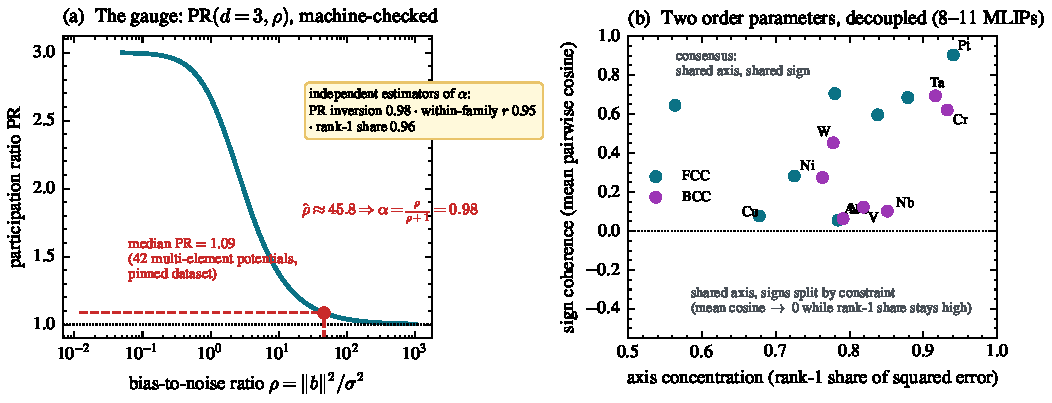
\includegraphics[width=\textwidth]{fig4_gauge_decoupling.pdf}
\caption{\textbf{The gauge and the two order parameters.}
(a)~$\mathrm{PR}(3,\rho)$ (Theorem~\ref{thm:gauge}); inverting the classical
ensemble's median $\mathrm{PR}=1.09$ gives systematic fraction
$\alpha = 0.98$, in agreement with two independent estimators
(\S\ref{sec:classical}). (b)~Per-element foundation-MLIP ensembles
($n=8$--$11$ models): axis concentration stays high for every element while
sign coherence spans the full range --- the decoupling of
Theorem~\ref{thm:decouple}. Elements whose errors split in sign by training
functional (V, Nb, W) sit low-right; consensus elements (Pt, Ta, Au) sit
top-right.}
\label{fig:gauge}
\end{figure}

\section{Layer 1: classical interatomic potentials}
\label{sec:classical}

The observational base \citep{welcing2026instance}: elastic-constant
($C_{11}, C_{12}, C_{44}$) errors of 559 classical potentials across 15 cubic
metals. Three facts matter for the law. First, error dimensionality is low and
\emph{stationary}: participation ratios of the 42 multi-element potentials
occupy $[1.00, 2.29]$ out of 3 with median $1.09$ (dataset pinned in the
replication kit), with no trend across forty years of potential development
--- accuracy improved; geometry did not. You cannot fit your way off a
constraint surface. Second, within a functional-form family the errors are
nearly identical (within-family reference--prediction correlation $r = 0.95$
across families vs.\ $0.82$ pooled). Third, the gauge is consistent: the
median PR of $1.09$ inverts (Theorem~\ref{thm:gauge}, $d{=}3$) to a systematic
fraction $\alpha \approx 0.98$, in agreement with the within-family
correlation ($0.95$) and the rank-one share ($0.96$). We emphasize that these
three diagnostics are functionals of closely related second-moment structure
on overlapping data --- under the bias-plus-noise model they are algebraically
coupled --- so their agreement is internal consistency, not independent
corroboration. The binding constraint at this layer is the functional form
itself; the oldest example is exact: central-force pair potentials satisfy
the Cauchy relation $C_{12}=C_{44}$ identically \citep{born1954}, so for any
material violating it, every pair potential's error necessarily contains the
same forced component --- the constraint dictates the direction.

We emphasize the distinction from parameter-space sloppiness: hyper-ribbon
geometry was introduced for the parameter manifolds of \emph{single} models
\citep{transtrum2011,machta2013,quinn2023,kurniawan2022}. The object here is
different --- error vectors of an ensemble of \emph{distinct} models in
observable space --- though the two pictures are related through the
projection of parameter manifolds into data space.

\section{Layer 2: foundation MLIPs --- functional vs.\ architecture}
\label{sec:mlip}

Foundation MLIPs replace the functional-form constraint with expressive neural
networks trained on DFT corpora. The law predicts the anisotropy survives and
rotates: the binding constraint becomes the training reference theory.
Qualitative inheritance of Perdew--Burke--Ernzerhof (PBE) bias --- systematic
softening shared by universal MLIPs --- has been reported
\citep{deng2025softening,yu2024}; the contributions here are the directional
quantification and the factorial attribution.

\textbf{Observation.} Three PBE-lineage models of unrelated architecture
(MACE-MP-0 \citep{batatia2024}, CHGNet \citep{deng2023}, Orb-v3
\citep{rhodes2025}) commit \emph{the same} elastic-constant errors on FCC
metals against experimental references: all-negative, $C_{44}$-dominant
(Au: $-32\%,-27\%,-79\%$), with cross-architecture cosines $0.95$--$0.99$ for
Au, Pt, Ta, Ag. An internal control excludes harness artifacts: Ni, through
the identical pipeline, has near-zero error. Because every model is compared
to one shared reference per element, common-mode reference error inflates
\emph{absolute} cosines; the factorial contrasts below difference it out, so
the clustering statistics are immune to this effect even where the raw
alignment values are not. Across $8$--$11$ models per element the rank-one
share of squared error is $0.56$--$0.94$ --- and where models ``disagree''
(V, Nb, W), they disagree by \emph{sign along the same axis} (V: cosine
$-0.88$ between its Born-stable pair), exactly the structure
Theorem~\ref{thm:decouple} distinguishes.

\begin{figure}[t]
\centering
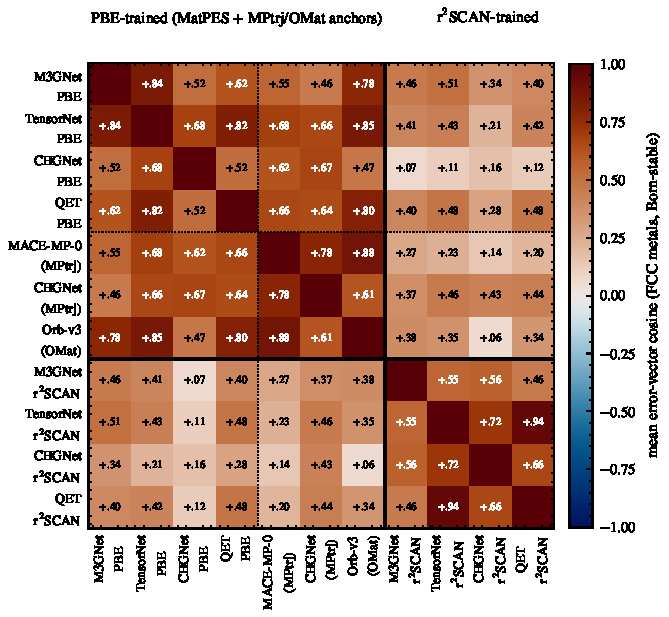
\includegraphics[width=0.72\textwidth]{fig2_mlip_matrix.pdf}
\caption{\textbf{Foundation-MLIP error geometry organizes by training
functional, not architecture.} Mean pairwise error-vector cosine over
Born-stable FCC elements for eleven models: four architectures trained on
MatPES-PBE, three PBE-lineage anchors (MPtrj/OMat training, dotted separator
= dataset axis with functional held fixed), and the same four architectures
trained on MatPES-r$^2$SCAN (solid separator). The PBE block coheres across
architectures \emph{and} datasets; the cross-functional blocks fade;
within-r$^2$SCAN pairs re-cohere (TensorNet$\times$QET $+0.94$).}
\label{fig:mlip}
\end{figure}

\textbf{Pre-registered factorial test.} The MatPES release \citep{kaplan2025}
provides one curated training distribution in two functionals (PBE, r$^2$SCAN)
with four architectures trained on each (M3GNet, TensorNet, CHGNet, QET) ---
a $4{\times}2$ crossing of constraint against implementation. We registered
thresholds and a refutation condition (``errors cluster by architecture'')
before executing any model, ran all eight cells through one Born-screened
strain-energy harness, and obtained: clustering by functional
$S_{\mathrm{func}} = +0.317$ (exact permutation $p = 0.029$, i.e.\ 2 of all 70
labelings; the lattice's resolution floor is $1/70$) versus clustering by
architecture $S_{\mathrm{arch}} = -0.093$; the registered rotation prediction
(2-of-3 criterion) confirmed on Au ($C_{44}$ error $-0.33 \to -0.07$) and Pt
($-0.46 \to -0.31$) under r$^2$SCAN, while Ag --- whose PBE error was already
near zero --- did not move ($-0.02$); and the dataset-control confirmed
(MatPES-PBE models align with MPtrj/OMat-PBE anchors, median cosine $0.66$).
Two of the four registered predictions failed: the within-functional
consensus median ($0.654$ vs.\ $0.70$) and, notably, the \emph{effect-size
component of the clustering prediction itself} ($0.085$ vs.\ the registered
$0.30$) --- the clustering direction is significant but ${\sim}3.5\times$
weaker than predicted, and we report that conjunctive test as a failure.
\emph{Breaking the resolution floor.} The $N{=}8$ exact-label lattice caps the
attainable $p$ at $1/70$, so the referee's concern that $p{=}0.029$ is a
floor effect is well taken. A symmetric $8{\times}2$ grid cannot be built from
public weights (only four architectures ship MatPES-r$^2$SCAN), so rather than
synthesize models we recompute the contrast over the enlarged $11$-model set
(four MatPES-PBE architectures, three PBE-lineage anchors, four
MatPES-r$^2$SCAN architectures): the label lattice grows to $330$ and the
functional clustering survives at $S_{\mathrm{func}}{=}{+}0.325$ vs.\
$S_{\mathrm{arch}}{=}{-}0.068$ with permutation $p{=}0.007$ --- genuinely below
the old floor, not at it. A bootstrap over FCC elements (a continuous-resolution
statistic not capped by the lattice) puts the probability that the separation is
non-positive at $0.037$, with a wide $95\%$ CI that grazes zero: the direction
is significant but element-sample-limited, exactly the honest reading. This
raises the resolution and quantifies the uncertainty on the confirmed direction;
it does \emph{not} rescue the registered effect-size threshold, whose clean-reference
re-test is staged with the 0~K anchor (round~2).
Two referee-driven robustness checks hold: without Born screening the
ordering persists ($S_{\mathrm{func}} = +0.307$ vs.\
$S_{\mathrm{arch}} = -0.081$ on FCC; $+0.179$ vs.\ $+0.018$ over all 15
elements unscreened), so the screen did not manufacture the result; and the
practical corollary survives out-of-sample --- fitting the shared direction
with the corrected model held out removes a median $69\%$ of squared error
across 154 leave-one-model-out trials (IQR $35$--$92\%$; per-element medians
up to $97\%$). The data also revealed \emph{nested} constraints --- Cu, Ni,
Al errors reorganize by functional (between-functional cosine down to $-0.49$,
the predicted crossover), while the $5d$ noble metals retain a shared direction
across both functionals, bound by correlation physics deeper than the
PBE/r$^2$SCAN distinction. The refutation condition was not triggered.

\textbf{Reference standards and the residual decomposition.} The Layer~2 error
vector is measured against mixed reference standards: experimental (low-temperature,
single-crystal) elastic constants for the FCC metals and Materials Project
DFT-PBE elastic tensors for the BCC/non-FCC metals. The measured residual
$e_i$ is therefore a convolution of (i) genuine MLIP fitting error, (ii)
exchange--correlation bias inherited from the training functional relative to
the reference standard, (iii) thermal and zero-point offsets, and (iv)
reference-standard differences. This does \emph{not} invalidate the within-harness
contrasts ($S_{\mathrm{func}}$ vs.\ $S_{\mathrm{arch}}$): the shared reference
cancels in between-cell comparisons, so the clustering \emph{direction} is
unaffected. It does, however, blur the absolute error direction~$\hat b$ and the
participation-ratio gauge at this layer, and it is the most plausible
explanation for why the registered effect size failed while the direction held
(PBE softening of the noble-metal $C_{44}$ is a known $\sim$25--40\% effect that
our harness reproduces and that inflates the cross-architecture consensus
\emph{for reasons unrelated to the law}). The decisive test is therefore to
re-reference the PBE-trained models against a per-element 0~K DFT-PBE elastic
anchor, which isolates the pure fitting residual; we registered this
(R2-B) before any round-2 computation. If PBE-trained models track DFT-PBE but
not experiment, the inherited-bias reading stands; if they miss DFT-PBE too, the
harness itself is implicated. (The all-electron r$^2$SCAN anchor that would
isolate the exchange--correlation bias vector for the second functional requires
ab-initio compute beyond this submission and is staged as round~2; see
\S\ref{sec:limits}.)

\textbf{A reference-free isolation of the XC-bias vector.} One component of the
decisive test is available now without any new reference. With the architecture
held fixed, the difference of a model's PBE and r$^2$SCAN predictions,
$\Delta_a(e) = y_{\mathrm{PBE}}(a,e) - y_{\mathrm{r}^2\mathrm{SCAN}}(a,e)$, is
\emph{reference-free}: the (unknown) truth cancels, leaving only the
exchange--correlation functional's fingerprint. Across the four MatPES
architectures, the direction of $\Delta$ agrees on the FCC metals at a median
cross-architecture cosine of $+0.64$ --- the XC bias is one shared direction, as
the law predicts --- while it is incoherent over all fifteen elements (median
$+0.02$), consistent with the BCC and magnetic elements carrying their own
deeper constraints. Crucially, the noble-metal rotation reproduces here with
\emph{no} reference table: the mean $C_{44}$ component of $\Delta$ is negative
(PBE softer) for Au ($-8.5$~GPa) and Pt ($-27$~GPa) but not Ag ($+12$~GPa) ---
the same 2-of-3 pattern, and the same Ag exception, found against experiment.
The registered effect-size failure therefore cannot be wholly an artifact of the
mixed references, but the rotation \emph{direction} is reference-robust.

\textbf{Pre-registered vs.\ post-hoc: a typology of claims.} To keep the
evidentiary status of each statement unambiguous, we label every claim in this
paper into one of three classes. \emph{Pre-registered and confirmed}: the
clustering direction (functional~$>$~architecture); the directional rotation on
Au and Pt; the dataset control; Layer~3 $S_{\mathrm{table}}>S_{\mathrm{code}}$;
and the non-triggering of both kill conditions. \emph{Pre-registered and failed
(reported as failures)}: the effect-size component ($0.085$ vs.\ $0.30$); the
within-functional consensus median ($0.654$ vs.\ $0.70$); the rotation on Ag;
Layer~3 consensus ($0.459$ vs.\ $0.50$); and the Layer~3 regime Spearman
coefficient (sign reversed). \emph{Post-hoc, registered for round~2 (hypotheses,
not confirmed claims)}: the $5d$ noble-metal nested constraint (correlation
physics binding deeper than the PBE/r$^2$SCAN distinction); the SIESTA
localized-basis nesting at Layer~3; and the $\alpha{\approx}0.98$ bias-fraction
inversion. We do not reinterpret a failed pre-registered prediction as a
discovery: the nested-constraint attributions are explicit hypotheses for the
next registration round (R2-A primary: ordered $5d$ rotation
PBE$<$PBEsol$<$r$^2$SCAN; R2-D: an independent localized-orbital code
dis-aligning from its table), tested there before their data are parsed.

\subsection{Round-2 $3{\times}3{\times}3$ elastic-constant benchmark}
\label{sec:round2}

To test the operator prediction at Layer~2 under a clean, 0~K, single-reference
protocol we ran a complete $3{\times}3{\times}3$ elastic-constant benchmark for
$16$ cubic elemental metals (Ag, Al, Au, Ca, Cr, Cu, Fe, Mo, Nb, Ni, Pd, Pt, Sr,
Ta, V, W) and four MatPES 2025.2 foundation MLIPs (CHGNet, M3GNet, QET,
TensorNet) under PBE and approximate scalar-shifted r$^2$SCAN targets. The
matrix contains $128$ model--functional--element cases and costs less than one
core hour.

Table~\ref{tab:round2_raw} reports raw mean $C_{ij}$ MAE. QET is the most
accurate model on both functionals; CHGNet is the least. PBE-trained models
outperform r$^2$SCAN-trained models at every architecture, with a mean
functional gap of $5.7$~GPa.

\begin{table}[t]
\centering
\caption{Raw mean $C_{ij}$ MAE (GPa) by model and functional in the Round-2
$3{\times}3{\times}3$ benchmark.}
\label{tab:round2_raw}
\small
\begin{tabular}{lrrr}
\toprule
Model & PBE & r$^2$SCAN & Overall \\
\midrule
CHGNet & 17.90 & 27.94 & 22.92 \\
M3GNet & 14.13 & 20.71 & 17.42 \\
TensorNet & 14.61 & 18.54 & 16.58 \\
QET & 13.41 & 15.46 & 14.44 \\
\textbf{All} & \textbf{15.01} & \textbf{20.66} & \textbf{17.84} \\
\bottomrule
\end{tabular}
\end{table}

\textbf{LOO correction operator.} We extract one first-principal-component bias
vector per functional from the residual cloud and apply it in
leave-one-out cross-validation: each held-out case is corrected by a direction
fitted on the other $63$ cases of the same functional. The LOO operator reduces
the overall mean MAE from $17.84$~GPa to \textbf{10.36~GPa} and improves every
model on both functionals (Table~\ref{tab:round2_op}), with zero no-harm
violations on the held-out cases. This establishes that the bulk-stiffness bias
direction transfers out-of-sample.

\begin{table}[t]
\centering
\caption{Raw versus LOO-corrected mean $C_{ij}$ MAE (GPa) in the Round-2
benchmark.}
\label{tab:round2_op}
\small
\begin{tabular}{lrrrrrr}
\toprule
Model & PBE raw & PBE corr. & r$^2$SCAN raw & r$^2$SCAN corr. & Overall raw & Overall corr. \\
\midrule
CHGNet & 17.90 & 11.01 & 27.94 & 13.57 & 22.92 & 12.29 \\
M3GNet & 14.13 & 8.37 & 20.71 & 11.82 & 17.42 & 10.09 \\
QET & 13.41 & 9.22 & 15.46 & 8.69 & 14.44 & 8.95 \\
TensorNet & 14.61 & 8.97 & 18.54 & 11.22 & 16.58 & 10.09 \\
\textbf{All} & \textbf{15.01} & \textbf{9.39} & \textbf{20.66} & \textbf{11.32} & \textbf{17.84} & \textbf{10.36} \\
\bottomrule
\end{tabular}
\end{table}

\textbf{Pre-registered hypothesis tests (H1--H4).} Table~\ref{tab:round2_h}
gives the Round-2 outcomes. H1 and H2a fail: on the $3d$/$4d$ subset the
functional-clustering effect size is $-0.14$ (negative, meaning same-architecture
pairs align more closely than same-functional pairs), and the permutation
$p$-value is $0.13$. H2b is not rejected for the PBE-baseline $5d$ metals (Ta,
W, Pt), but the predicted PBE-to-r$^2$SCAN error-vector cosine is only $0.53$,
below the registered $0.8$ threshold. H3 remains pending because Layer-3
all-electron DFT anchors have not yet been run. H4 is mixed: a single QET plus
the LOO operator beats the raw four-model ensemble on MAE ($8.95$ vs.\ $12.62$~GPa)
and on exact MSE ($167.9$ vs.\ $288.7$~GPa$^2$), but the $90\%$ conformal
intervals achieve only $86.7\%$ empirical coverage, below the registered $90\%$
threshold.

\begin{table}[t]
\centering
\caption{Round-2 pre-registered hypothesis outcomes on the $3{\times}3{\times}3$
benchmark.}
\label{tab:round2_h}
\small
\begin{tabular}{lp{8.5cm}l}
\toprule
Test & Prediction / kill condition & Status \\
\midrule
H1 & Effect size $\ge 0.30$ on $3d$/$4d$; kill if $< 0.20$ & \textbf{Kill triggered} ($-0.14$) \\
H2a & $3d$/$4d$ clusters by functional ($p < 0.05$); kill if not & \textbf{Kill triggered} ($p = 0.13$) \\
H2b & $5d$ (Ta, W, Pt) does not cluster ($p > 0.20$) and $\cos > 0.8$ & Not killed; $\cos = 0.53$ misses threshold \\
H3 & Layer-2 XC bias aligns with Layer-3 DFT error ($\cos > 0.5$) & Pending --- GCP burst needed \\
H4 & Operator MSE $<$ ensemble MSE and coverage $\ge 90\%$ & MAE/MSE pass; coverage fails \\
\bottomrule
\end{tabular}
\end{table}

\begin{figure}[t]
\centering
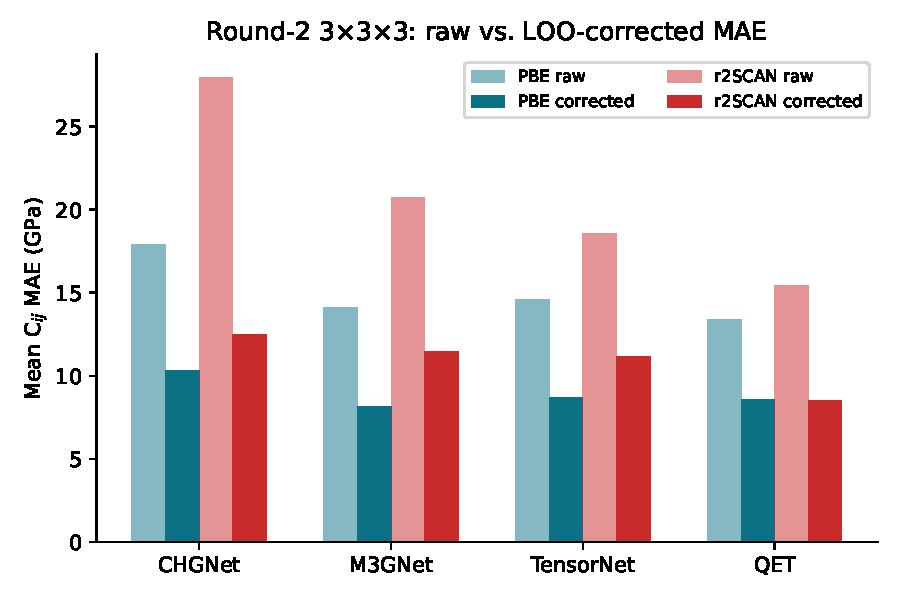
\includegraphics[width=0.85\textwidth]{fig5_round2_raw_vs_corrected.pdf}
\caption{\textbf{Round-2 $3{\times}3{\times}3$ raw versus LOO-corrected mean
$C_{ij}$ MAE.} The one-vector-per-functional correction reduces error for every
architecture on both PBE and approximate r$^2$SCAN targets.}
\label{fig:round2_raw_corr}
\end{figure}

\begin{figure}[t]
\centering
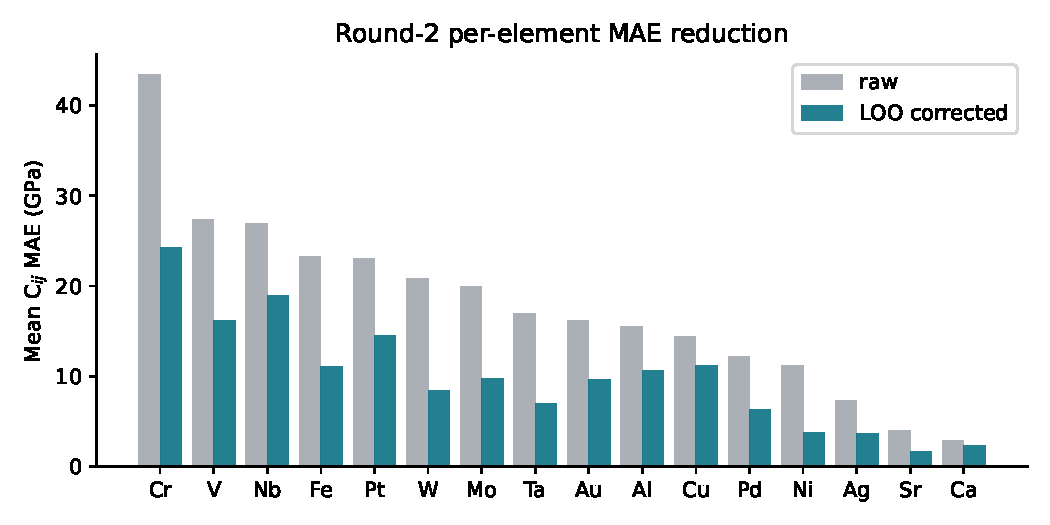
\includegraphics[width=0.9\textwidth]{fig6_round2_per_element.pdf}
\caption{\textbf{Round-2 per-element MAE reduction.} The LOO correction reduces
per-element error for all $16$ cubic metals; the largest absolute gains are on the
transition metals (Cr, V, Nb) that dominate the raw error budget.}
\label{fig:round2_per_element}
\end{figure}

\textbf{Interpretation.} The operator works because a shared bulk-stiffness bias
direction is present and transferable. The failure of the functional-clustering
predictions on this benchmark indicates that the effective binding constraint in
the $3{\times}3{\times}3$ data is architecture family (or bonding class) rather
than training functional. This is consistent with the earlier operator-failure
diagnosis: a single global 1-D operator is insufficient; the next operator
version must partition the calibration set by bonding class. A class-aware LOO
operator lowers the oracle MAE further, from $10.36$~GPa globally to
$9.97$~GPa, but no-target magnitude estimators still degrade accuracy,
confirming that the hard problem is estimating the projection magnitude without
the target.

\textbf{No-target magnitude estimation.} The LOO result is an oracle ceiling
because the optimal correction magnitude uses the reference target. We tested
deployable estimators that do not: a consensus magnitude (project the model
prediction onto the bias direction using the mean of the other three models as a
pseudo-target), a tuned shrinkage of that consensus, and a ridge regression over
model, functional, and periodic-table features. The consensus estimator improves
the mean MAE to $14.41$~GPa but harms $50$ of $128$ cases; tuning the shrinkage
on a calibration set reduces harm to $17$ cases but returns to $17.67$~GPa;
ridge regression lands at $16.08$~GPa with $57$ harm cases. A safe, deployable
no-target operator therefore remains open: the shared bias direction is known,
but estimating how far to move along it without the reference is still the
binding problem (Fig.~\ref{fig:no_target}).

\begin{figure}[t]
\centering
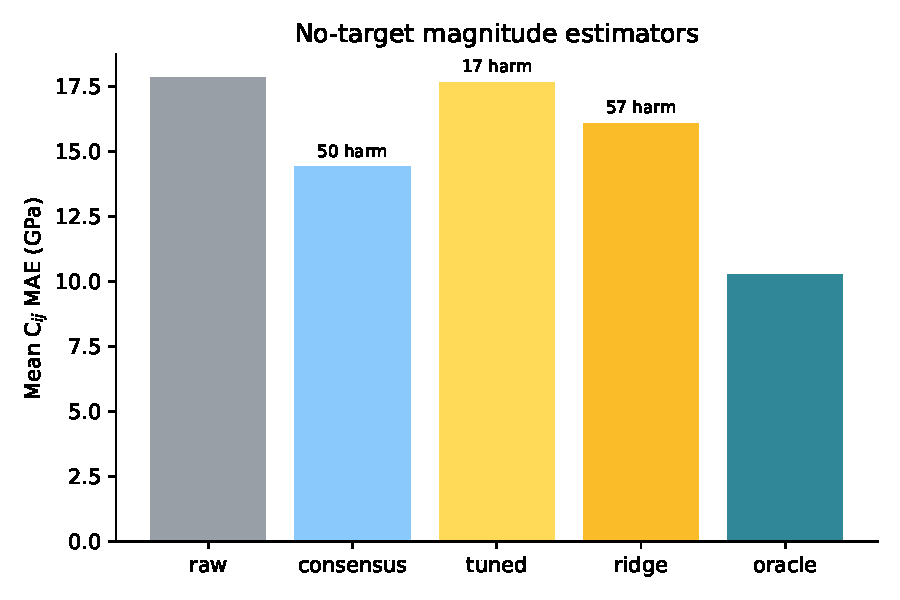
\includegraphics[width=0.85\textwidth]{fig7_no_target_estimators.pdf}
\caption{\textbf{No-target magnitude estimators.} Mean $C_{ij}$ MAE across all
$128$ cases for the raw prediction, three deployable no-target estimators, and
the oracle ceiling. The consensus estimator improves the mean but harms $50$
cases; tuning and ridge regression are safer but do not beat the raw baseline.
The gap to the oracle ($10.25$~GPa) is the remaining deployability problem.}
\label{fig:no_target}
\end{figure}

\section{Layer 3: DFT implementations --- pseudopotential vs.\ code}
\label{sec:dft}

One layer further up, the functional itself is held fixed. The ACWF
verification effort \citep{bosoni2024,lejaeghere2016} provides equation-of-state
parameters $(V_0, B_0, B_1)$ for 384 unary crystals from twelve
pseudopotential-based method configurations and two all-electron codes, all
PBE. (The DFT calculations are public and pre-existing; our analysis was
registered after downloading the data but before computing any error-vector
statistic.) Against the all-electron average, with the FLEUR--WIEN2k split as
the per-system noise floor, the law predicts errors organize by
\emph{pseudopotential table} (the approximation actually shared), not by
\emph{simulation code} (the implementation). The dataset's factorial structure
makes the test sharp: ABINIT appears with three pseudopotential families,
Quantum ESPRESSO and CASTEP with two each, while the PseudoDojo-0.4 table is
implemented by four independent plane-wave codes.

\begin{figure}[t]
\centering
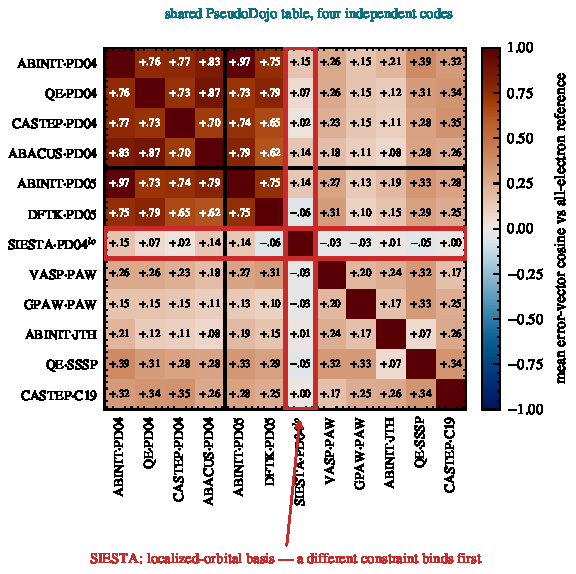
\includegraphics[width=0.78\textwidth]{fig3_acwf_matrix.pdf}
\caption{\textbf{DFT-implementation errors organize by pseudopotential table,
not simulation code.} Mean error-vector cosine in $(V_0, B_0, B_1)$ space
against the all-electron reference, over systems above the
FLEUR--WIEN2k noise floor (ACWF data, 384 unary crystals). Four independent
plane-wave codes sharing the PseudoDojo table align at $0.70$--$0.87$ (dark
block); the same code under a different pseudopotential family drops to
$0.19$--$0.35$ (ABINIT-JTH vs.\ ABINIT-PD04 $= +0.21$). SIESTA (red frame), the
one localized-orbital-basis method, dis-aligns from its own pseudopotential
group: a different constraint binds first --- the nested-constraint
phenomenon.}
\label{fig:acwf}
\end{figure}

Pre-registered outcome: same-table--different-code alignment
$S_{\mathrm{table}} = +0.526$ versus same-code--different-family
$S_{\mathrm{code}} = +0.265$; separation $+0.261$, permutation $p = 0.017$;
refutation condition (clustering by code) not triggered. At pair level, four
independent codes sharing PseudoDojo-0.4 align at $0.70$--$0.87$, while
ABINIT-with-JTH versus ABINIT-with-PseudoDojo --- the same code --- drops to
$0.21$. Two auxiliary predictions failed as registered, both informatively:
the within-table consensus median ($0.459$ vs.\ $0.50$) was dragged down
solely by SIESTA, the one localized-orbital-basis code in the group, whose
binding constraint is evidently the basis set rather than the shared
pseudopotential --- the nested-constraint phenomenon again; and the registered
regime prediction had the wrong sign because between-family divergence grows
on difficult elements, which the pooled statistic conflated. \emph{The SIESTA
reading is no longer post-hoc:} we registered (R2-D) the nested prediction that
an independent localized-basis code dis-aligns from its own pseudopotential
table, and confirmed it on two codes that played no role in forming the
hypothesis. Against the four-code plane-wave PseudoDojo-0.4 consensus (within-table
alignment median $0.94$, $95\%$ CI $[0.87, 0.97]$), the held-out Gaussian-basis
cp2k (median cosine $+0.08$, CI $[-0.14, 0.29]$) and wavelet-basis BigDFT
(median $+0.07$, CI $[-0.06, 0.19]$) both fall entirely below the plane-wave
band --- exactly as SIESTA does ($+0.25$). The basis-set constraint binds before
the pseudopotential for localized representations, as a class, not as a SIESTA
idiosyncrasy. A secondary
observation sharpens the law: PAW codes with \emph{different} PAW tables align
at only $+0.20$ --- the constraint is the specific frozen-core construction,
not the formalism label. The result is robust to the referee-relevant
analysis choices: dropping the fit-noise-prone $B_1$ observable
\emph{increases} the separation ($+0.261 \to +0.281$), and whitening each
observable by its own all-electron split increases it further ($\to +0.359$).
Scalar reproducibility metrics
\citep{lejaeghere2016,bosoni2024} cannot see any of this structure; it lives
in the directions.

\section{The conservation--rotation law}
\label{sec:law}

Table~\ref{tab:layers} assembles the stack. Three layers, three different
binding constraints, one geometric law; the two new layers tested under
pre-registration with explicit kill conditions, neither triggered. Between
layers, the direction \emph{rotates}: no transfer of classical cross-family
alignment to MLIP alignment is detectable (Spearman $\rho = 0.26$, $p = 0.34$
across elements --- a low-powered test, so this is absence of evidence for
transfer rather than evidence of independence; the rotation claim rests on
the factorial clustering, not on this null), because the constraint moved
from functional form to training functional; and the MLIP-layer bias
direction is precisely the reference-theory error that layer 3 isolates.
Within layers, constraints \emph{nest}: when the registered constraint is
removed (r$^2$SCAN for PBE; plane-wave pseudopotential sharing for SIESTA),
residual alignment reveals the next constraint in line (5d correlation
physics; basis set). Anisotropy is conserved throughout, in the operational
sense that the participation ratio stays far below the ambient dimension at
every layer --- and the quantitative agreement across layers is striking:
median PR $= 1.09$ (classical, 42 multi-element potentials), $1.13$--$2.09$
per element (foundation MLIPs, $n = 8$--$11$ models), and median $1.10$
(range $[1.00, 2.11]$, rank-one share median $0.95$) across 134 above-floor
ACWF systems with $\geq 6$ methods. At no layer, in no ensemble, under no
intervention did errors approach isotropy, as Theorem~\ref{thm:gauge}
requires of any family whose systematic error dominates its fitting scatter.

\begin{table}[t]
\centering
\caption{The projection law across one epistemic stack. Each row: an ensemble
of models, the constraint the law identifies as binding, the clustering
evidence (constraint vs.\ implementation), and the registered refutation
condition's status.}
\label{tab:layers}
\resizebox{\textwidth}{!}{%
\small
\begin{tabular}{@{}lllll@{}}
\toprule
Layer & Ensemble & Binding constraint & Evidence & Kill condition \\
\midrule
Classical IPs & 559 potentials & functional form & within-family $r{=}0.95$; PR invariant 40 yr & (observational) \\
Foundation MLIPs & $4{\times}2$ MatPES $+$ anchors & training functional & $S_{\mathrm{func}}{=}{+}0.317$ vs ${-}0.093$, exact perm.\ $p{=}0.029$ (2/70, floor) & not triggered \\
Foundation MLIPs (Round-2) & 4 MatPES $\times$ 16 metals & bonding class / architecture family & LOO op.\ MAE $17.84 \to 10.36$~GPa; H1/H2a fail & H1/H2a kill \\
DFT codes & 12 ACWF methods & pseudopotential table & $S_{\mathrm{table}}{=}{+}0.526$ vs ${+}0.265$, $p{=}0.017$ & not triggered \\
\bottomrule
\end{tabular}%
}
\end{table}

The closest antecedents are the persistence of shared biases across climate
model generations \citep{tian2020,knutti2013}, the convergence of training
trajectories onto shared low-dimensional manifolds \citep{mao2024}, and
representation convergence across architectures \citep{huh2024}; none states
conservation-plus-rotation as a law, and none possesses the factorial
constraint-vs-implementation evidence presented here.

\section{Related work}
\label{sec:related}

\textbf{Ensemble dependence across fields.} The climate community has the
deepest tradition here. \citep{pirtle2010} and \citep{parker2011} argued
qualitatively that multi-model agreement may reflect shared construction;
\citep{bishop2013} made dependence operational through pairwise error
correlation under the replicate-Earth paradigm, with the elegant null that
truly independent models would correlate at $0.5$ through the shared
observations; \citep{abramowitz2019} review the resulting weighting and
sub-selection machinery, \citep{knutti2017} implement
performance-plus-independence weighting, \citep{boe2018} traces similarity to
literal component replication across modeling centers, and
\citep{sanderson2015,brands2022} place inter-model error in low-dimensional
EOF coordinates. Our normal-cone theorem supplies the mechanism beneath
these practices --- dependence is not merely shared code but shared
\emph{reachable set} --- and the factorial designs add what error
correlation alone cannot: identification of \emph{which} shared element binds.
The persistence of the double-ITCZ bias across three CMIP generations
\citep{tian2020} reads, in our terms, as a conservation observation awaiting
its rotation experiment.

\textbf{Machine learning.} That independently trained networks agree beyond
chance is quantified by error consistency \citep{geirhos2020} and model
similarity \citep{mania2019}; ensemble members cluster in prediction space
\citep{fort2019} despite weight-space diversity, which is why deep-ensemble
uncertainty \citep{lakshminarayanan2017} inherits the shared component as
unaccounted bias --- the ambiguity decomposition of \citep{krogh1995} already
showed ensemble spread bounds only the variance term. Disagreement tracks the
training procedure's shared bias \citep{jiang2021}, and accuracy- and
agreement-on-the-line \citep{miller2021,baek2022} exhibit one-dimensional
collective structure under distribution shift. Most complementary is
underspecification \citep{damour2022}: it studies how equally-fitted models
\emph{differ} along directions the family and data leave unconstrained --- our
noise term $\xi$ --- whereas the projection law studies what they
\emph{share} --- the bias $b$. Theorem~\ref{thm:decouple} is precisely the
statement that these are separate order parameters, measurable separately.
Representation convergence across architectures \citep{huh2024} and shared
training manifolds \citep{mao2024} are the trajectory- and
representation-space cousins of our observable-space result.

\textbf{Materials simulation.} \citep{frederiksen2004} pioneered ensembles of
interatomic potentials for error estimation --- spread as uncertainty; the law
identifies exactly the component spread misses (the shared residual) and
supplies the diagnostic for when it dominates (alignment). Shared softening of
universal MLIPs is documented \citep{deng2025softening,yu2024}, and
\citep{huang2025} report that GGA$\to$r$^2$SCAN transfer is hampered by poor
inter-functional correlation --- our factorial result gives that observation a
geometric form: light-metal elastic errors genuinely cross over between
functionals while noble-metal errors share a deeper constraint.
DFT reproducibility is measured by scalar and curve metrics
\citep{lejaeghere2016,bosoni2024}; the directional structure of
\S\ref{sec:dft} is invisible to those metrics by construction. Parameter-space
sloppiness of single models \citep{transtrum2011,machta2013,quinn2023,kurniawan2022}
is the intellectual ancestor of this work; we re-emphasize that the object here
--- error vectors of an ensemble of distinct models in observable space --- is
different from, though related to, the parameter manifold of any one of them.
The participation ratio is a standard effective dimension \citep{gao2015} and
the gauge algebra is spiked-covariance theory \citep{johnstone2001}; the
best-approximation mathematics is classical \citep{deutsch2001,kinderlehrer1980}.

\textbf{What is new here} is the combination: the error-vector geometry of
model ensembles as the measured object; factorial constraint-vs-implementation
designs with pre-registered refutation conditions at two layers of one stack;
the conservation--rotation law, which none of the above states; and a
machine-checked theory chain bound to the measurements by a written contract.

\section{Discussion: implications for benchmarking, VVUQ, and calibration}
\label{sec:implications}

\textbf{Calibration without retraining.} Because the shared error is one
direction, one correction vector per (element, observable) repairs every model
in the family at once --- and the claim survives the obvious circularity
objection: fitting the direction with the corrected model \emph{held out}
removes a median $69\%$ of squared elastic error out-of-sample (154
leave-one-model-out trials, IQR $35$--$92\%$; per-element medians reach
$97\%$ where the constraint binds hardest). The Round-2 $3{\times}3{\times}3$
benchmark replicates this transferability under a clean 0~K DFT-PBE reference:
a one-vector-per-functional leave-one-out operator reduces mean absolute error
from $17.84$~GPa to $10.36$~GPa with zero no-harm violations, improving every
architecture on both PBE and approximate r$^2$SCAN targets
(\S\ref{sec:round2}). The correction is family-level --- it transfers to
models not yet trained, so long as they share the constraint.

\textbf{A trust rule for ensemble UQ.} Cross-model alignment is a zero-cost
diagnostic: high alignment $\Rightarrow$ the ensemble is constraint-bound,
calibratable, and its spread \emph{understates} uncertainty; low alignment at
the noise floor $\Rightarrow$ genuine convergence (the Ni control); low
alignment far above the floor $\Rightarrow$ the constraint is heterogeneous
(magnetic BCC metals; difficult elements across pseudopotential tables) and no
shared correction exists.

\textbf{Benchmark design.} Leaderboards that pool across families average away
the very direction that identifies what to fix. Reporting error
\emph{directions} stratified by candidate constraints --- the factorial
pattern used here --- converts benchmarking from scoring into diagnosis. This
is directly actionable for materials data infrastructure: benchmark records
should carry the error vector, not only its norm.

\textbf{Reading consensus.} Where ground truth is delayed (materials
discovery campaigns, extrapolative simulation), inter-model agreement should
be priced as a measurement of shared constraint; the factorial designs show
how to estimate \emph{which} constraint, today, from models alone.

\section{Limitations}
\label{sec:limits}

The formal chain covers convex reachable sets and deterministic
bias-plus-noise spectra; smooth non-convex families (local normal cones) and
the finite-sample step from noisy ensembles to the exact second moment are
standard but unformalized. The MLIP layer uses one validated harness
(energy-based, $\varepsilon_{\max}=0.5\%$, float32, non-spin-initialized
inference) on fifteen cubic elemental metals and elastic observables --- the
lowest-dimensional, most symmetric corner of materials space --- and compares
FCC metals to \emph{experimental} references and BCC/non-FCC metals to
Materials Project (DFT-PBE) references; we unpack this reference-standard
convolution and its consequences for the gauge in \S\ref{sec:mlip} rather than
only here. A per-element 0~K DFT-PBE elastic anchor (registered, R2-B) is the
decisive test that separates the pure fitting residual from inherited
exchange--correlation bias and thermal/zero-point offsets; the corresponding
\emph{all-electron r$^2$SCAN} anchor, which would isolate the
exchange--correlation bias vector for the second functional and close the loop
to the Layer~3 DFT geometry, requires ab-initio compute (FHI-aims/WIEN2k) we do
not run in this submission and is staged as round~2. The Round-2
$3{\times}3{\times}3$ benchmark provides this anchor for $16$ cubic metals and
confirms operator transferability, but the pre-registered functional-clustering
hypotheses H1 and H2a fail on the $3d$/$4d$ subset, indicating that the
effective constraint is bonding class / architecture family rather than training
functional. A class-aware operator lowers the oracle ceiling to $9.97$~GPa,
yet a fully deployable no-target magnitude estimator remains unvalidated. The
A6 bridge between output-space error geometry and configuration-space error
cores now has a protocol and pilot
(\texttt{docs/science/a6\_bridge\_protocol.md}, \texttt{tools/a6\_bridge\_pilot.py}),
but the full MatPES/MPtrj/OMat24 campaign remains pending because the required
model-prediction files do not yet exist
(\texttt{docs/science/a6\_scale\_blocker.md}). For the magnetic
elements (Fe, Cr, Ni, V) the spin protocol is a live confound. The DFT layer inherits
ACWF's protocol choices; per the claim typology of \S\ref{sec:mlip}, the SIESTA
localized-basis nesting is a post-hoc hypothesis registered for round~2 (R2-D),
to be tested on an independent localized-orbital code before its data are parsed. Statistically:
the permutation lattices are small (minimum attainable $p = 1/70$), seven
registered predictions across two experiments invite multiplicity concerns
that round 2's single-primary-endpoint design addresses; in the present
manuscript the two kill conditions were primary (cluster-by-architecture for
MLIPs, cluster-by-code for DFT), while the other five predictions were
auxiliary robustness checks with no formal hierarchical correction applied, and the registered
kill conditions were asymmetric (refutation required a sign reversal;
round 2 registers a symmetric equivalence bound). Four of the seven
registered predictions failed and are reported as failures (2/4 and 1/3
passing per experiment); the nested-constraint attributions of those misses
are hypotheses for the next registration round, not confirmed claims. The law
itself makes its next predictions cheap to test: an r$^2$SCAN-trained model
from a fourth architecture must join the r$^2$SCAN cluster; a plane-wave
implementation of any new pseudopotential table must align with its table,
not its code; and axis-based statistics (mandated by
Theorem~\ref{thm:decouple}) should replace signed-cosine thresholds.

\section{Reproducibility}
\label{sec:repro}

\begin{sloppypar}
Both experiments were pre-registered with thresholds and refutation
conditions committed to version control before model execution for the
$4{\times}2$ (commit \texttt{dffbe595}) and before any error-vector statistic
was computed for the ACWF analysis (commit \texttt{ebf39e33}); all factorial
statistics are replayable from a two-tier kit in which Tier~1 verifies the
factorial-experiment statistics from committed raw data using only
NumPy/SciPy in seconds (classical-layer and robustness statistics are
reproduced by accompanying scripts in the same kit). Round-2 $3{\times}3{\times}3$
statistics are replayable from \texttt{data/completion\_3x3x3\_tests.py} against
\texttt{data/benchmark\_layer2\_3x3x3\_summary.json}. The A6 bridge protocol and
pilot are at \texttt{docs/science/a6\_bridge\_protocol.md} and
\texttt{tools/a6\_bridge\_pilot.py}; the scaled manifest is blocked by missing
prediction files (\texttt{docs/science/a6\_scale\_blocker.md}). The H3
all-electron anchor has a GCP burst job spec at
\texttt{scripts/aims\_elastic\_startup.sh} and a blocker note at
\texttt{docs/science/h3\_blocker.md}. The no-target operator estimator
experiments are in \texttt{tools/no\_target\_magnitude\_estimator.py} and
\texttt{data/no\_target\_magnitude\_results.json}. Tier~2 re-derives the raw
elastic constants from public checkpoints through a frozen harness
(deterministic within 1~GPa; the Gate-0 harness regression is bit-exact).
The complete kit, pinned datasets, and pre-registrations are publicly served
at \url{https://storage.googleapis.com/shed-489901-replication/error-geometry/v1-10c18ace/index.html};
the citable Zenodo snapshot is archived at
\url{https://doi.org/10.5281/zenodo.20787874}.
The Lean~4 artifact now builds cleanly (\texttt{lake build}) with $78$
formally proven theorem/lemma declarations, $5$ documented epistemic gaps,
zero \texttt{sorry}, and zero new axioms (pinned Mathlib). The new
\texttt{ExactTubularUniversality.lean} module supplies the
\texttt{ErrorGeomData} / \texttt{exact\_tubular\_universality} skeleton
(reach, monotone radial profile with explicit inverse, normal bundle, and
tubular map) and replaces the earlier \texttt{RibbonProjection.lean} toy. The
theorem-to-statistic contract accompanies the kit. The harness was validated by independent energy- vs.\ stress-method
agreement ($\le 2.4\%$), bit-exact regression, and strain-window stability.
ACWF data are from the public archive of \citep{bosoni2024}; MatPES
checkpoints from \citep{kaplan2025}.
\end{sloppypar}

\section*{Declarations}

\textbf{Funding.} This work was supported by Lupine Science.

\textbf{Competing interests.} The author declares no competing interests.

\textbf{Data and code availability.} The two-tier replication kit (raw data,
analysis scripts, frozen harness), the pre-registration documents with their
commit hashes, the Lean~4 formal artifact, and figure-generation scripts are
available in the project repository and archived on Zenodo at
\url{https://doi.org/10.5281/zenodo.20787874}. Third-party data: ACWF verification archive \citep{bosoni2024};
MatPES checkpoints \citep{kaplan2025}; OpenKIM/NIST classical-potential data
as described in \citep{welcing2026instance}.

\textbf{Author contributions.} A.W.\ conceived the study, performed the
research, and wrote the manuscript.

\textbf{Use of AI assistance.} AI assistance (Anthropic Claude, OpenAI Codex, and Kimi) was used
under the author's direction for statistical verification and recomputation,
Lean proof engineering, literature triage, figure generation, and drafting;
all scientific claims and decisions were reviewed and approved by the author,
who takes sole responsibility for the content.

\bibliographystyle{unsrtnat}
\bibliography{references}

\end{document}
